
\chapter{DEVELOPMENT OF A MULTIPLE-MINIMA FLUCTUATING CHARGE (MM-FLUCQ) POTENTIAL FOR PLATINUM-OXIDE FORMATION}
\label{chap:mmFlucQ}


In this chapter a brief overview of charge transfer methods will be presented
alongside the initial development of the mm-FlucQ potential.  Preliminary
results of charged species approaching a \ce{Pt} surface will also be
examined. Finally, current challenges and future directions will be discussed.

%polarization near metal surfaces
% drude model
% charge transfer

\section{Introduction}
Metal surfaces and interfaces play a key role in a number of chemical and
technological processes; however, the tendency of oxide layers to form on these
interfaces requires a chemically-realistic treatment of metal-adsorbate interactions when
simulating these systems\citep{Streitz:1994mw, Duin:2010dk, Devine:2011bk,
Fantauzzi:2014pb}.  The modified atomistic structure and electronic environment
of these surfaces after oxide formation is expected to affect many properties
of the interface, especially the local electric field, and also diffusion and
adsorption on the surface.\citep{Streitz:1994mw, Getman:2008sp,
Bray:2011hq,Small:2012dw}

Treating the charge transfer dynamics of such a system within molecular dynamics is a
challenging problem. Whereas non-metallic species can be modeled satisfactorily
with static point charges, metal-adsorbate, metal oxide, and more generally
metal-metal interactions require a more complicated description of their
electronic interactions to accurately capture the behavior of charged
species near a conductor. The idea of electronegativity equalization introduced
by Sanderson\citep{Sanderson:1951mz} provides a conceptual framework that
describes charge transfer between both atomic and molecular species. In this
formalism, as a species gains negative charge in response to its local
environment, its electronegativity decreases; similarly, if an atomic site has
lost charge, then it has an increased electronegativity. The system would then
only be considered at equilibrium if all of the electronegativities were equal.
It is helpful to remember that the electronegativity, $\chi_A$, as defined by
Mulliken\citep{Mulliken:1934wt} is equal to the negative of the chemical
potential of the valence electron gas around a positive nucleus, $\mu_A$, as
argued by Iczkowski and Margrave\citep{Iczkowski:1961wq}.

\begin{equation}
\chi_A = -\mu_A = -\frac{\partial E}{\partial q}
\end{equation}

In this equation $E$ is the ground state energy of the atom while $q$, the net
charge of the atom, is equal to $n - Z$ where $Z$ is the atomic number and $n$
is the number of electrons around the nucleus. Thus $q = 0$ for the neutral
species, $+1$ for the positive ion, and $-1$ for the negative ion.  This
description implies that upon movement of the nuclei, the electrons will
undergo charge transfer so as to equilibrate the electrochemical potential of
the system. While this formalism is helpful, it still requires a method
of implementation.  Streitz and Mintmire, using the idea of electronegativity
equalization, developed a potential for modeling aluminum oxide. They
calculated the minimum charges at each time step by taking the inverse of an
$n\times n$ matrix, which while accurate, drastically increases the expense of a simulation.\citep{Streitz:1994mw} A method proposed by Rick {\it et
al.} in their work on fluctuating charge water models is able to avoid matrix inversion by
allowing the atomic charges to fluctuate dynamically. This was accomplished by
coupling the electronegativity equalization method with a fictitious charge
variable on each atomic site. This charge variable $Q_A$ was then propagated
with the rest of the dynamics of the system by using an extended Lagrangian
approach.\citep{Rick:1994ss}

The basic idea of a dynamic fluctuating charge model is to allow partial
charges on atomic sites to become dynamical variables.  Each atomic site
therefore has four ``position'' variables, $\{\vec{\mathbf{r}}_A, Q_A\}$, and
four velocities, $\{\dot{\vec{\mathbf{r}}}_A, \dot{Q}_A\}$.   In addition to
standard electrostatic interactions between the fluctuating charges, there is a
self energy term that must be taken into account. Similar to Rapp\'e and
Goddard\citep{Rappe:1991dq} we can make use of a Taylor expansion around the
neutral atomic species with respect to charge.  This self term through second
order leads to,

\begin{equation} \label{eqn:selfenergy}
E_A(Q_A) = E_{A_0} + Q_A\bigg( \frac{\partial E}{\partial Q} \bigg )_{A_0} +
\frac{1}{2}Q_A^2 \bigg(\frac{\partial^2E}{\partial Q^2}\bigg)_{A_0}
\end{equation}

where $E_{A_0}$ is the ground state energy of the neutral species, $A$, and the
higher order terms are shown to be the electronegativity, $\chi$, and
electronic hardness, $J$, as derived below,

\begin{align*}
\mathrm{IP} &= E_A(+1) - E_A(0) \\
& = E_{A_0} + \bigg (\frac{\partial E}{\partial Q}\bigg)_{A_0} + \frac{1}{2}\bigg(\frac{\partial^2E}{\partial Q^2}\bigg)_{A_0} - E_{A_0} \\
\mathrm{EA} &= E_A(0) - E_A(-1) \\
& = E_{A_0} - E_{A_0} + \bigg (\frac{\partial E}{\partial Q}\bigg)_{A_0} - \frac{1}{2}\bigg(\frac{\partial^2E}{\partial Q^2}\bigg)_{A_0}  \\
\bigg (\frac{\partial E}{\partial Q}\bigg)_{A_0} &= \frac{\mathrm{IP+EA}}{2} = \chi_A ,\qquad \bigg (\frac{\partial^2 E}{\partial Q^2}\bigg)_{A_0} = \mathrm{IP-EA} = J_A
\end{align*}

where IP is the ionization potential and EA is the electron affinity of species
$A$.  Note that this approach assumes the surface is smooth in the +1
\rightarrow -1 charge domain. This description allows us to rewrite equation
\ref{eqn:selfenergy} as the following,

\begin{equation}
E_A(Q_A) = E_{A_0} + \chi_A Q_A + \frac{1}{2} J_{A} Q_A^2
\label{eq:harmonic}
\end{equation}

The electronegativity $\chi$, when described as the average of the ionization
potential and electron affinity, enjoys some agreement with experimentally-derived properties; whereas a
definition of electronic hardness is best understood using Rapp\'e and
Goddard's approach, where $J$ is equal to the Coulomb overlap integral between
Slater orbitals centered on each atomic site\citep{Rappe:1991dq}.

The harmonic self energy, shown in equation \ref{eq:harmonic} is enormously useful.
Even in large systems of coupled fluctuating charge sites, the charges move on
a purely harmonic ``bowl'' where the minimum energy state for the system of
charges can be determined uniquely. Charge conservation constraints can be
applied to a constrained electronegativity equalization procedure to find the
best set of charges for a given set of nuclear positions.  Additionally, motion
of the atomic sites simply changes the location of the minimum and curvature of
the charge bowl, but these are relatively smooth variations, allowing standard
integration techniques to be used to propagate the charge variables.

One limitation of the harmonic self-interaction potential is the inability to
represent multiple stable oxidation states of various species. In many simple
molecules or ions, only one dominant oxidation state is present, but at the
surfaces of metals (and particularly during metal oxide formation), there can
be multiple oxidation states (e.g. \ce{Pt^0}, \ce{Pt^2+}, \ce{Pt^4+}, etc.)
present in the system simultaneously.

Another weakness of the harmonic approach is the reliance on the unit charge
gas phase ions in determining the first and second derivative terms, $\chi$ and
$J$.  In many charge partitioning schemes (and in most classical force fields),
the partial charges assigned to condensed phase atoms are significantly smaller
than the unit charges required to produce the gas phase ions, e.g. the \ce{H}
in \ce{H2O} in TIP4P is assigned a charge of +0.52.\citep{Jorgensen:1983tp}
This results in electronegativity and hardness terms that may estimate the
local slope and harmonic constants leading to construction of a charge surface
that is overly broad.

The method we present here builds on the fluctuating charge method of Rick {\it
et al.}\citep{Rick:1994ss}, but models the self energy more generally using
multiple stable ionic states.  This multiple-minimum fluctuating charge method
(mm-FlucQ) effectively allows for charge transfer between ionic and metallic
species.

\section{Development of methodology}

As we present the development of this approach, it is helpful to see how it
will fit into the total Lagrangian of the system. Similar to Rick {\it et
al.}\citep{Rick:1994ss} our Lagrangian is shown below,

\begin{equation}
L = \sum^{N_{molec}}_{i=1}\sum^{N_{atom}}_{\alpha = 1} \frac{1}{2}m_{\alpha} \dot{r}^2_{i\alpha} + \sum^{N_{molec}}_{i=1}\sum^{N_{atom}}_{\alpha = 1} \frac{1}{2}M_Q\dot{Q}^2_{i\alpha} - U[(\mathbf{Q}),(\mathbf{r})] - \lambda \sum^{N_{molec}}_{i=1}\sum^{N_{atom}}_{\alpha = 1} Q_{i\alpha}
\end{equation}

where the mass of an atomic site $\alpha$ is defined as $m_\alpha$ and $M_Q$ is
the fictitious charge mass with units of $\frac{\mathrm{energy\times
time}^2}{\mathrm{charge}^2}$.  The $\lambda$ term at the end of the Lagrangian
allows us to enforce total charge conservation in the system.

The potential energy term $U[(\mathbf{Q}),(\vec{\mathbf{r}})]$ contains the
expected pieces from standard molecular dynamics simulations,
$U_{\text{bonds}}, U_{\text{bends}}, U_{\text{torsions}},
U_{\text{electrostatics}}, U_{\text{van der Waals}}$ etc. It also contains the
new self energy term necessary for modeling dynamic fluctuating charges. This
term, instead of using the harmonic approximation, includes multiple diabatic
charge states,

\begin{equation}
U(Q) =
\begin{Bmatrix}
 V_0(Q) & c  \\
 c   & V_1(Q)
\end{Bmatrix}
\end{equation}

Where $c$ is a coupling constant between states $i$ and $j$, and $V_i(Q)$ is
seen below,

\begin{equation*}
V_i(Q) = \frac{1}{2}k(Q - Q_i)^2 + V_i
\end{equation*}

For each diabatic state, $V_i(Q)$ treats the local energy around a stable charge
site, $Q_i$, as a harmonic function with local curvature $k$ and offset by $V_i$.
By constructing our self-potential energy landscape out of many
diabatic states, we are able to create a surface with multiple charge minima.
An ideal multiple-well potential is shown in Figure \ref{fig:multipleDiabat}.
This method can be trivially extended by adding more diabatic states.

\begin{figure}
  \centering
  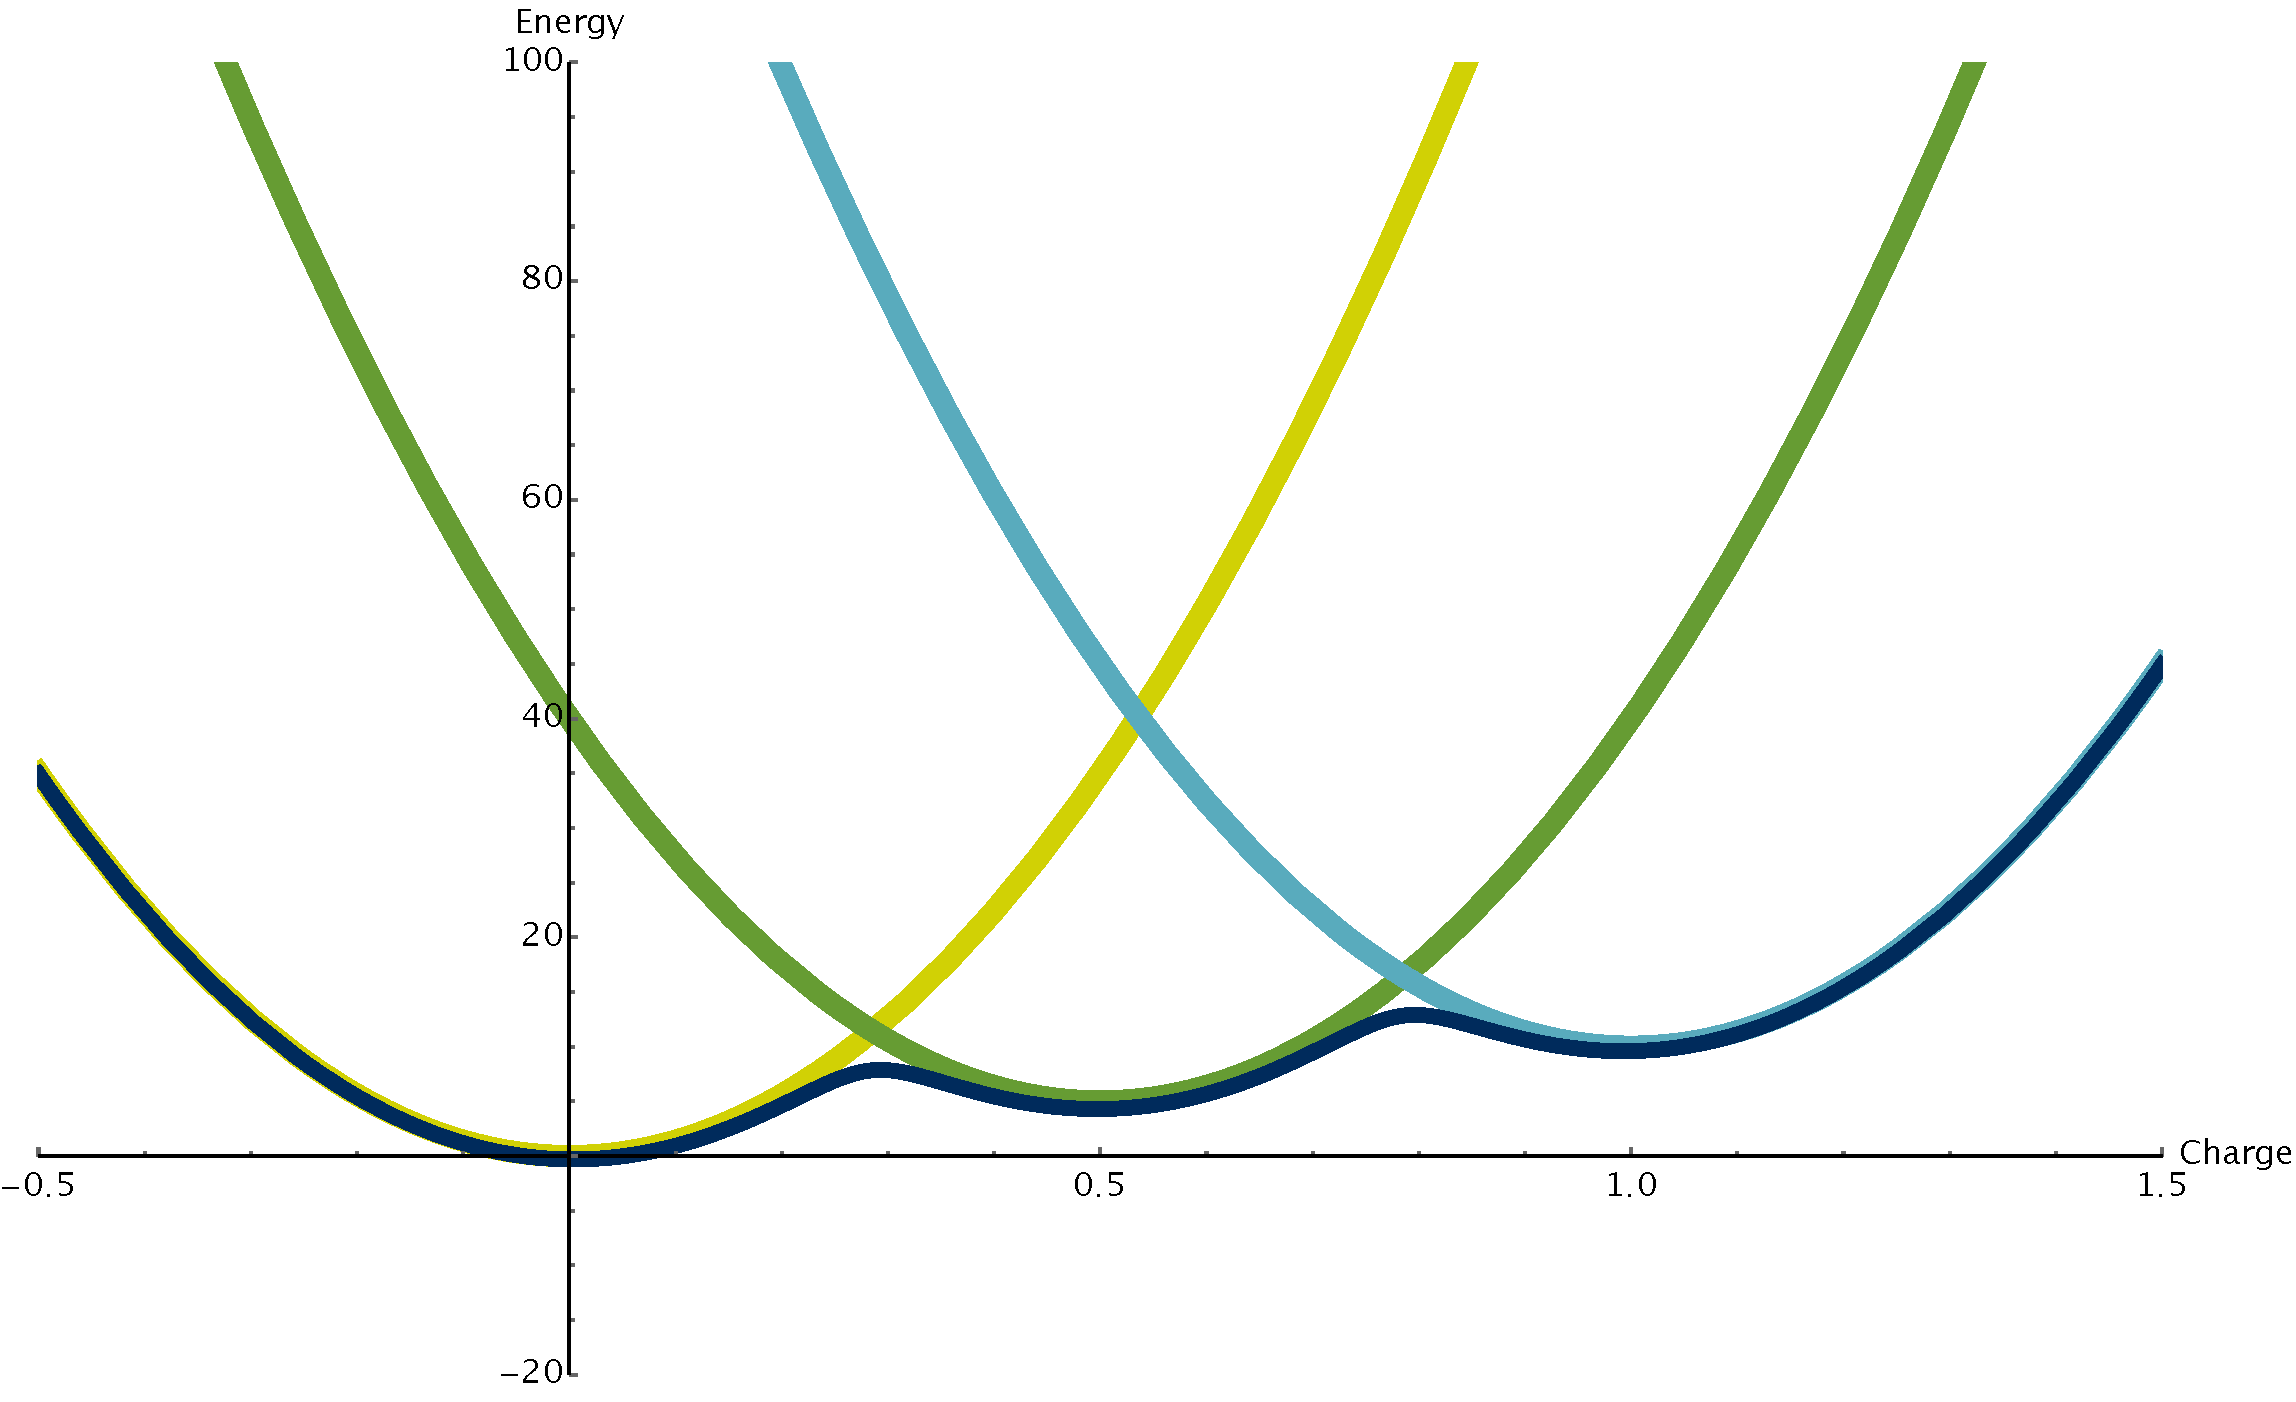
\includegraphics[width=0.75\linewidth]{../figures/chap5/multipleDiabats.pdf}
  \caption{The gold, green, and cyan curves represent the diabatic energies
that compose the navy triple-well adiabatic potential surface which is defined
using the following parameters and solving for the eigenvalues of the matrix.
$[Q_0 = 0, Q_1 = 0.5, Q_2 = 1, V_0 = 0, V_1 = 5, V_2 = 10, k = 280, c = 3.5]$}
\label{fig:multipleDiabat}
\end{figure}

\begin{equation*}
  \begin{Bmatrix}
    V_0(Q) & c      & 0      & \dots  & 0\\
    c      & V_1(Q) & c      & \dots & 0\\
    0      & c      & V_2(Q) & \ddots & 0 \\
    \vdots & \vdots & \ddots & \ddots & c\\
    0      & 0      & 0      &  c     & V_n(Q) \\
    \end{Bmatrix}
\end{equation*}

\subsection{Parameterization}
One weakness of this proposed method is the need for a large number of
parameters.  Currently, even with assumptions made about a single coupling
constant $c$, no coupling between states when $|i-j| > 1$, and $k$ being the
same for all of the individual diabatic states, there will still need to be
$2n+2$ parameters for $n$ diabatic states. 

\begin{equation*}
\text{Parameters} = [Q_0 \dots Q_n, V_0 \dots V_n, k, c] = \text{2n+2}
\end{equation*}

\subsubsection{Platinum \& Oxygen self-potentials}
A more complicated example then the above ideal surface, is the electronic surfaces
of oxygen and platinum in a platinum-oxide system.  The ``stable'' charge
position of the wells were obtained from a set of DFT calculations performed on
the platinum oxide surface. Bader charge analysis was performed and a histogram
was generated based on the populations of oxygen and platinum in various charge
states. The population analysis of both species is shown in Figure
\ref{fig:population} and a first attempt at the interaction potentials were
then created and are shown in Figures \ref{fig:Ocharge} and \ref{fig:PtCharge}.
The current approach attempts to minimize the effects of the bulk \ce{Pt} when
determining relative barrier heights between charge states.

\begin{figure}
  \centering
  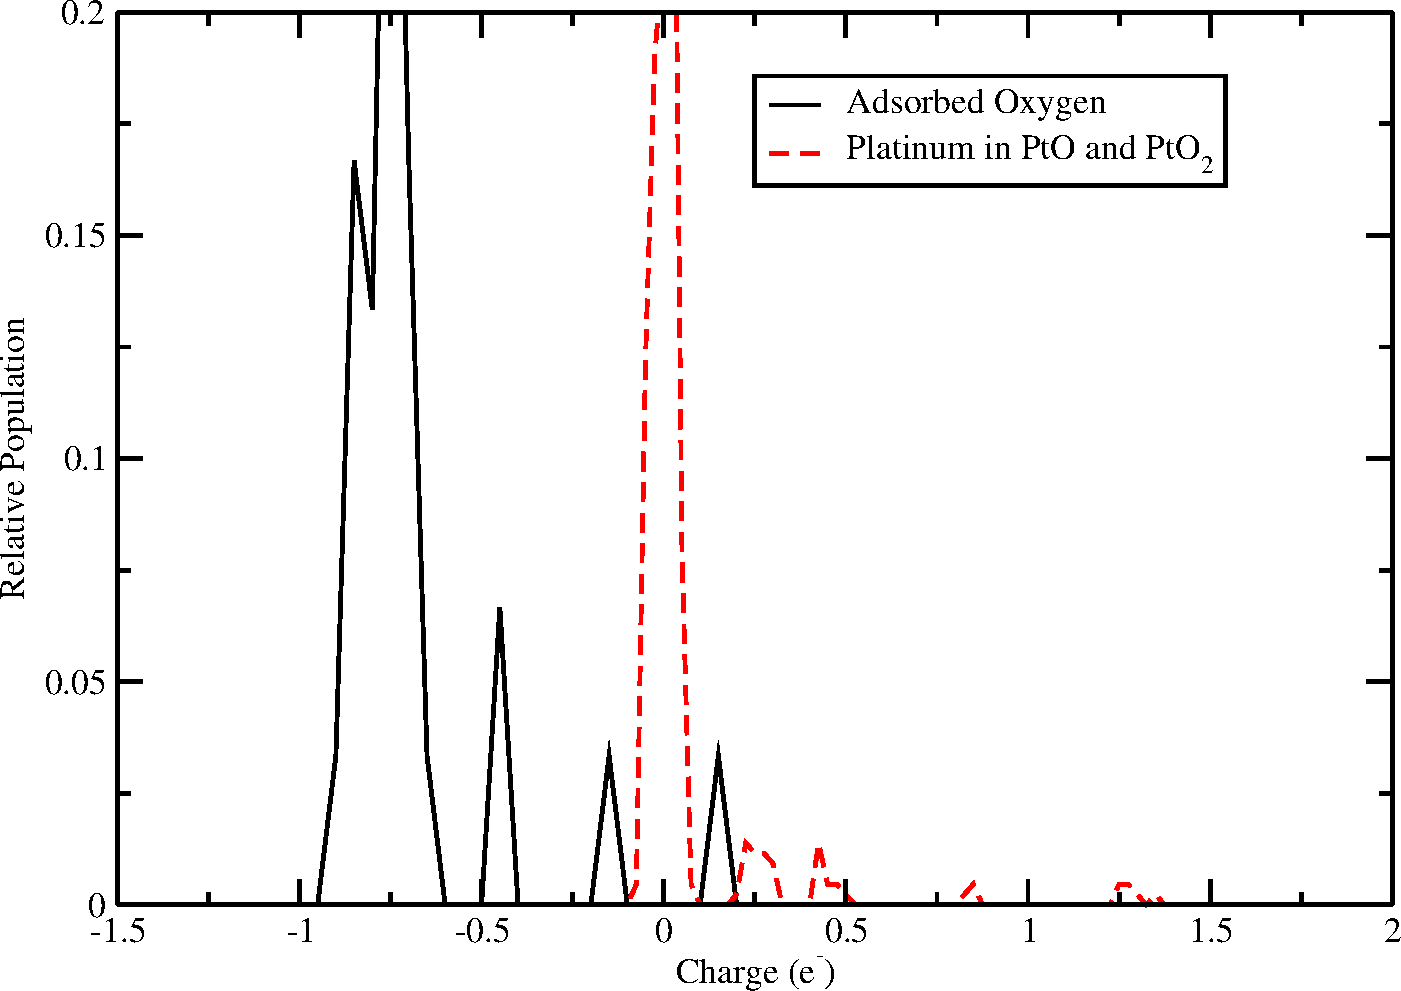
\includegraphics[width=0.75\linewidth]{../figures/chap5/chgDist_PtO.pdf}
  \caption{Histogram of oxygen (black, solid) and platinum (red, dashed)
charges obtained from a sampling of platinum oxide DFT calculations.
Normalization is proportional to number of atoms in the simulation, hence the
large peak centered around 0 for \ce{Pt}, since the majority of the metal is
unperturbed by surface \ce{O}.}
\label{fig:population}
\end{figure}

\begin{figure}
  \centering
  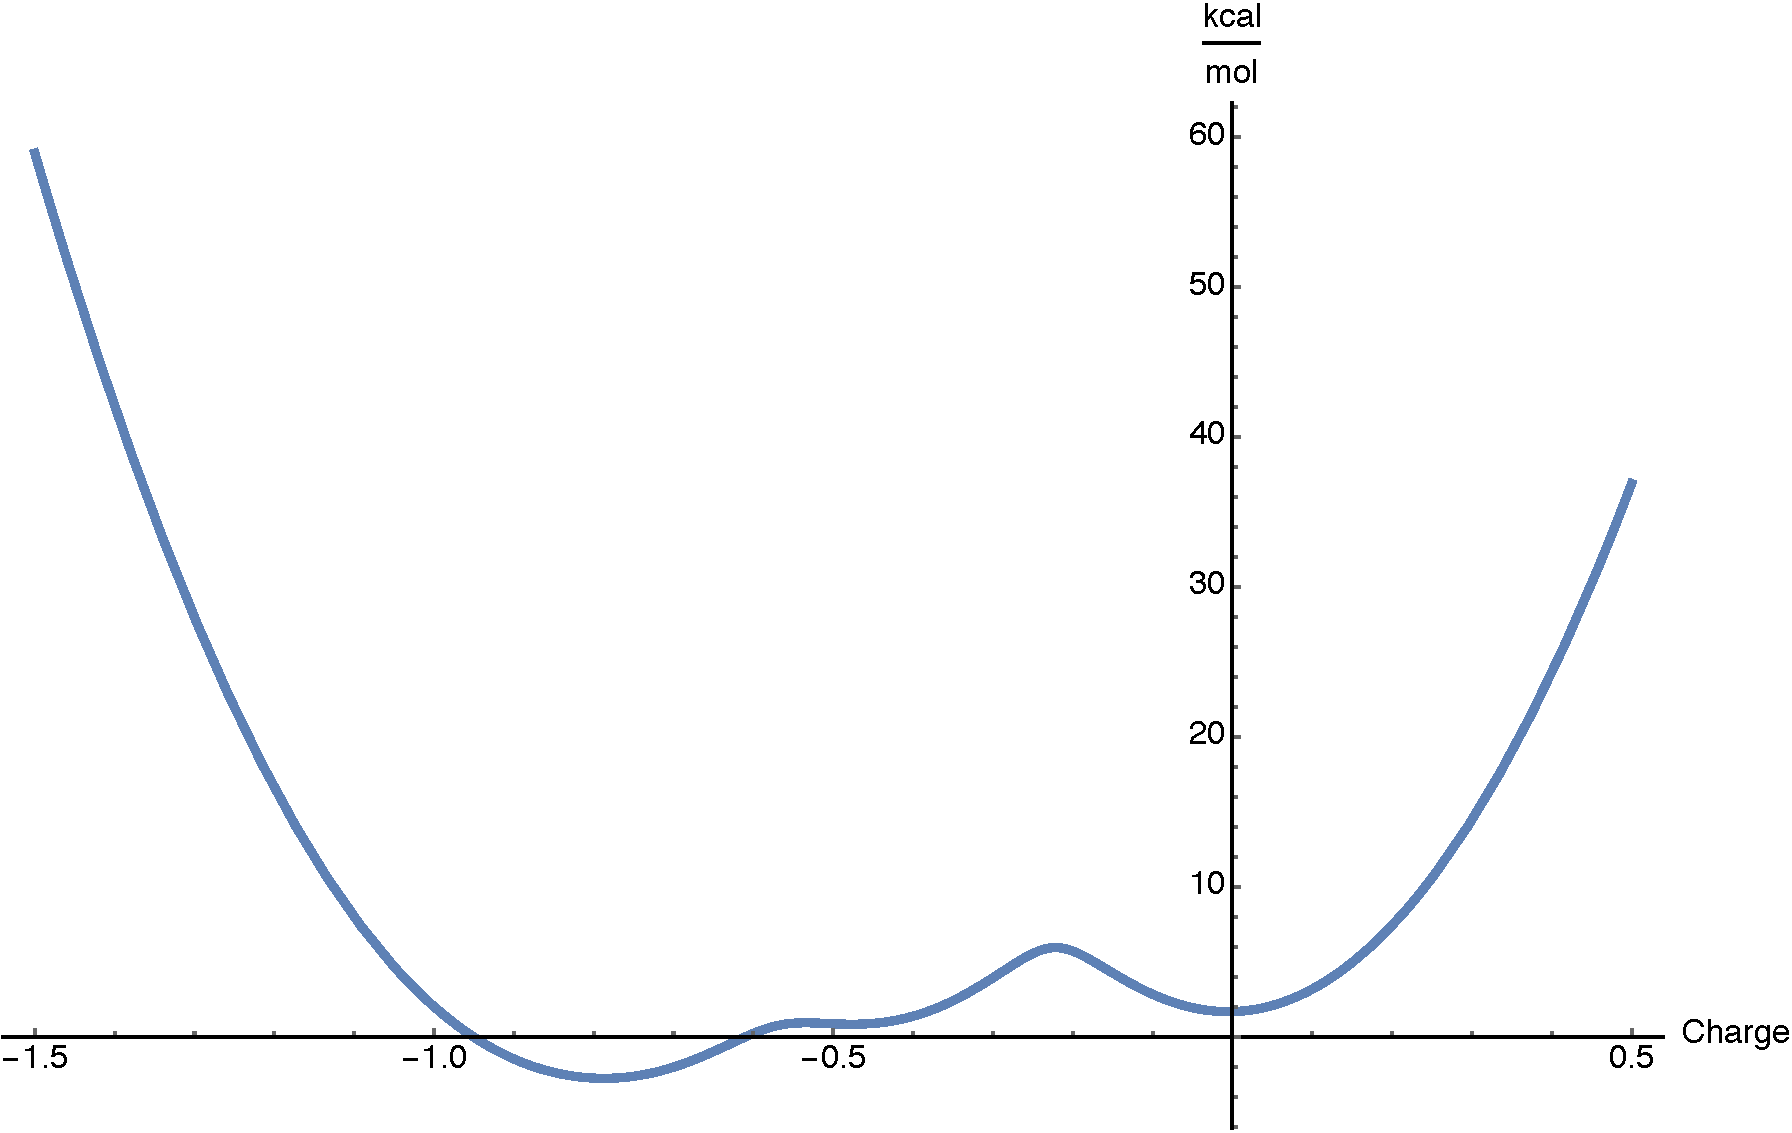
\includegraphics[width=0.75\linewidth]{../figures/chap5/Oxygen_Charge_Testing.pdf}
  \caption{A self-interaction oxygen charge potential. The parameters to
generate this potential are $[Q_0 = -0.85, Q_1 = -0.75, Q_2 = -0.45, Q_3 = 0,
V_0 = 0.25, V_1 = 0, V_2 = 2, V_3 = 2, k = 280, c = 3]$. As oxygen has a
favorable first ionization energy, it was decided that the global minimum
would be located around that point in this fit.}
\label{fig:Ocharge}
\end{figure}

\begin{figure}
  \centering
  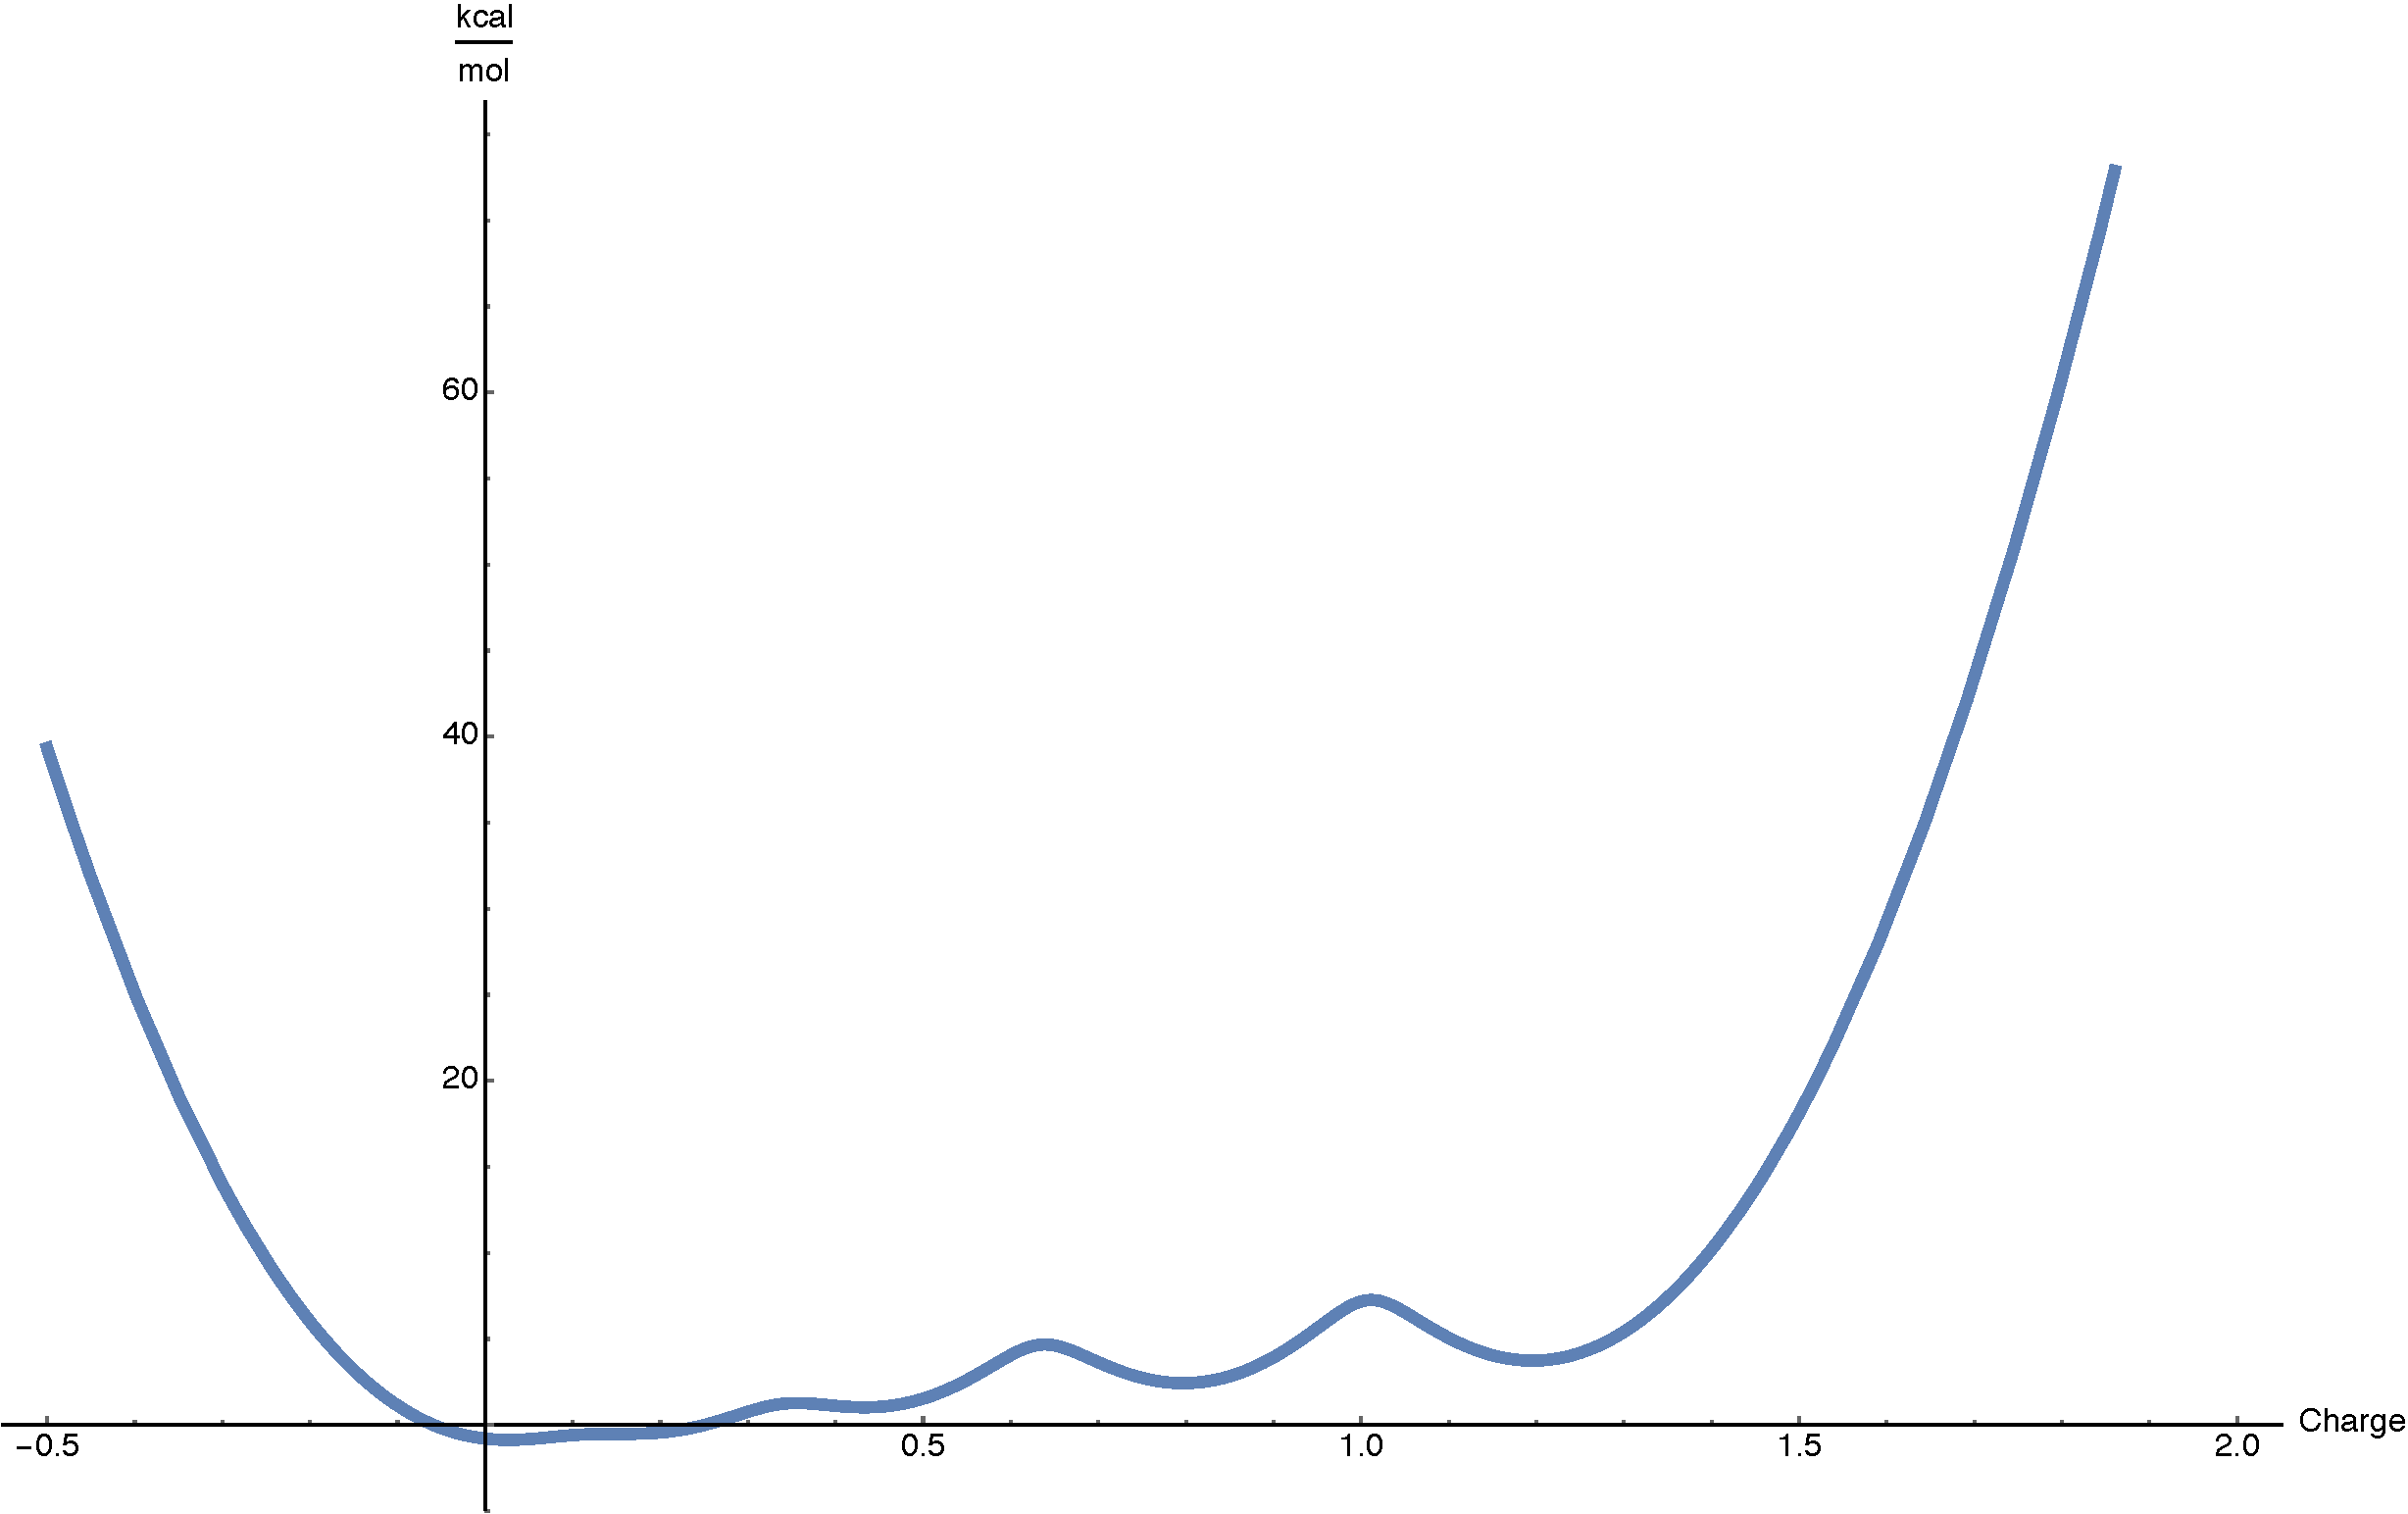
\includegraphics[width=0.75\linewidth]{../figures/chap5/Pt_Charge_Testing.pdf}
  \caption{A self-interaction platinum charge potential. The parameters to
generate this potential are $[q_0 = 0, q_1 = 0.2, q_2 = 0.45, q_3 = 0.8, q_4 =
1.2, V_0 = 0, V_1 = 1, V_2 = 2, V_3 = 3, V_4 = 4, k = 316, c = 2.5]$.}
\label{fig:PtCharge}
\end{figure}

Using the population analyses to determine valid charge states allows us to
parameterize the $Q_n$ values. The coupling constant $c$ currently has no
experimental justification and is tuned to ensure that a smooth potential is
obtained to minimize issues with integrating the dynamics. The scaling constant
$k$ has been obtained from the atomic/molecular polarizability by using an
ideal two particle system and is explained more fully in the next section.
Finally, the relative energies $V_n$ are currently being arbitrarily set until
we are able to provide theoretical or experimental justifications.

While the potentials in Figure \ref{fig:Ocharge} and \ref{fig:PtCharge} capture
some of the complexity of \ce{Pt\bond{-}O} interactions, for initial fitting
purposes self-energy potentials with 2 and 3 diabatic states are being used for
\ce{O} and \ce{Pt} to minimize the number of needed parameters.

\subsection{Derivation of k}
To determine the value for $k$, the scaling parameter in this scheme, we first
created an ideal two-particle system separated by $a_o$, as illustrated in
Figure \ref{fig:kSketch}.  We then arbitrarily shifted one unit of charge
between the otherwise identical atoms. The Hamiltonian of the system is
described below,

\begin{figure}
  \centering
  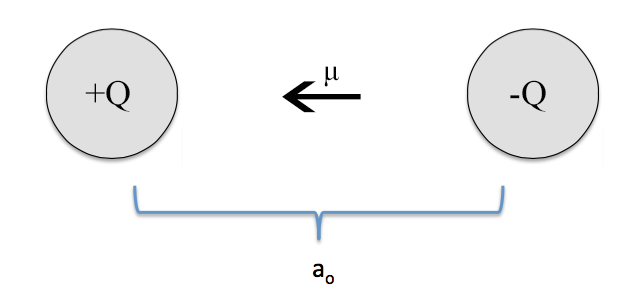
\includegraphics[width=0.75\linewidth]{../figures/chap5/determineK2.png}
  \caption{An ideal system of two particles with a forced charge separation of
$Q$ separated by a distance $a_o$. Constructing the Hamiltonian of this system
allows for a derivation of $k$.}
\label{fig:kSketch}
\end{figure}

\begin{equation*}
H = f_1(+Q) + f_2(-Q) - \frac{Q*Q}{4\pi\varepsilon_o a_o} - \mu\cdot\vec{E}
\end{equation*}

where $f_n(Q)$ describes the kinetic and simplified self-potential of the
atom's charge and is shown below,

\begin{equation*}
f(Q) = \frac{P_Q^2}{2m_Q} + \frac{1}{2}kQ^2
\end{equation*}

The ``charge momentum'' is represented by $P_Q$ and the ``charge mass'' by $m_Q$, while
$k$ is the scaling factor we are deriving. The electrostatic interaction term
and the dipole moment of the system interacting with the local electric field
complete the description of our model. Joining and rewriting the kinetic terms as $T$,
combining like terms, and replacing the dipole moment $\mu$ with $Q\cdot a_o$ leads to the
following,

\begin{equation*}
H = T + Q^2\bigg(k - \frac{1}{4 \pi\varepsilon_o a_o}\bigg) - Q\cdot a_o \cdot \vec{E}
\end{equation*}

The right two terms can be expressed as a shifted harmonic oscillator and can be solved in the
following manner after replacing $k-\frac{1}{4\pi\varepsilon_o a_o}$ with $a$
and $a_o\cdot \vec{E}$ with $b$.

\begin{equation*}
T + aQ^2 - bQ  = T + a\bigg(Q^2 - \frac{b}{a}Q\bigg) = T + a\bigg(\bigg(Q^2 - \frac{b}{a}Q + \frac{b^2}{4a^2}\bigg) - \frac{b^2}{4a^2}\bigg)
\end{equation*}

Taking the derivative of $H$ with respect to $Q$ to find the minimum results in $Q = \frac{b}{2a}$,
which when replacing $a$ and $b$ with their original values provides us with
the following equation for $Q_{\text{min}}$.

\begin{equation*}
Q_{\text{min}} = \frac{a_o \cdot \vec{E}}{2(k - \frac{1}{4\pi\varepsilon_o a_o})}
\end{equation*}

Recalling that the effective dipole moment is equal to $\mu_{\text{eff}} =
Q_{\text{min}}\cdot a_o$ and $\mu = \alpha\vec{E}$ where $\alpha$ is the atomic
polarizability, we reach the following solution for $k$.

\begin{equation*}
k = \frac{a_o^2}{2\alpha} + \frac{1}{4\pi\varepsilon_o a_o}
\end{equation*}

Using a polarizability for atomic Pt of $\alpha = 6.5$ \AA\textsuperscript{3}
and a nearest neighbor distance of $2.77$ \AA~ for bulk platinum we obtained a
value for $k$ of 316 $\frac{\text{kcal}}{\mathrm{mol\times e}^2}$. Various
polarizabilities and distances can be obtained for oxygen binding to platinum,
all leading to values for $k$ around 280 $\frac{\text{kcal}}{\mathrm{mol\times
e}^2}$.  These values are meant to be used as starting points for the
parameterization rather than as fixed points since the system used to derive
these values is an idealized model and not fully descriptive of the systems we
examined.

\section{Preliminary results}
As full parameterization is still underway, what follows is preliminary results
obtained during attempted parameterizations of forcefields for platinum oxide
systems. Specifically, one of the systems we model is composed of a negatively
charged oxygen atom approaching a (111) platinum surface. 
Since the mm-FlucQ method assume that a species electrons are collapsed
as point charges on the atomic sites, for the time being, anisotropy is not being considered. 

To visualize the charge density in these systems we begin by defining a uniform
grid of points (spacing approximately 1 \AA) spread throughout the simulation
box. The electron density as contributed by nearby atomic sites, assuming a
Gaussian distribution, is summed at each grid point and then assembled to use in
a volume rendering program, {\em e.g.} Amira. With regards to the electron
density, we treat density at a site $i$ with a three dimensional Gaussian
function as shown below,

\begin{equation*}
\rho(\vec{\mathbf{r}}) = \sum_i q_{i} \frac{1}{(2\pi)^{3/2}}e^{\frac{-(\vec{\mathbf{r}}-\vec{\mathbf{r}}_i)^2}{2}}
\end{equation*}

where our isotropic requirement leads to $\sigma_x = \sigma_y = \sigma_z = 1$,
$q_i$ is the charge of atom $i$ and $\Delta r$ is the distance from the point
where the density is being measured to the position of the atomic site
$\vec{\mathbf{r}}_i$. 

As seen in Figure \ref{fig:chargeVol}, which depicts an \ce{O-} ion approaching
a charge responsive \ce{Pt} surface, most of the metal atoms experience minimal
disruption away from the neutral ground state, whereas the metal directly
beneath the \ce{O-} ion gains a significant amount of positive charge. The
units of charge density are 0.001 $e^-$/\AA\textsuperscript{3} as calculated from the
above Gaussian. Figure \ref{fig:chargeHistogram} provides another view of this
system by looking at the charge population of the \ce{Pt} at various times over
the simulation length.

\begin{landscape}
\begin{figure}
  \centering
  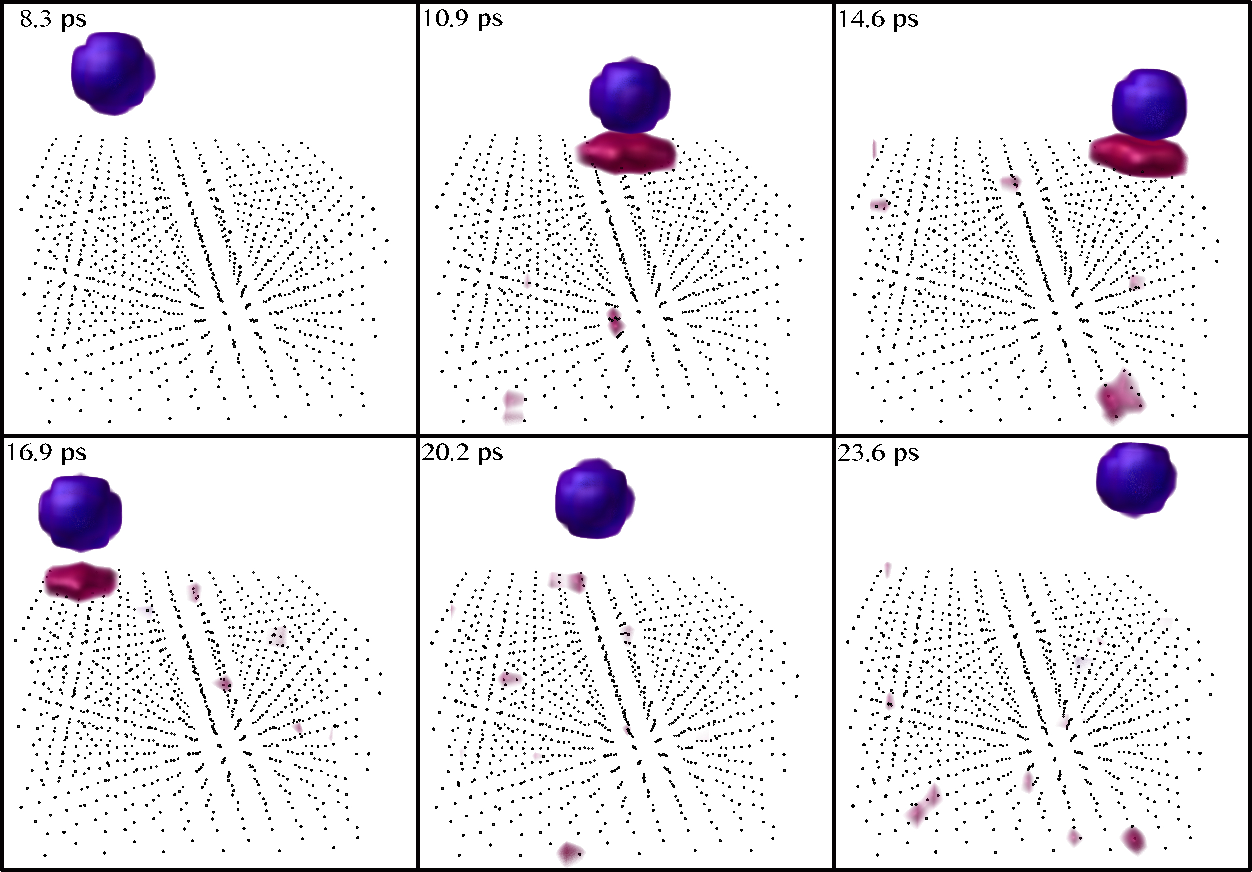
\includegraphics[width=0.7\linewidth]{../figures/chap5/PtOChargeVolume.pdf}
  \caption{As the \ce{O-} approaches the surface, the \ce{Pt} directly beneath
the \ce{O-} loses electron density leading to a favorable interaction between
the \ce{Pt} and \ce{O-}. Units are in $0.001\ e^-$/\AA\textsuperscript{3},
however only the extremes of charge are rendered.}
\label{fig:chargeVol}
\end{figure}
\end{landscape}

\begin{figure}
  \centering
  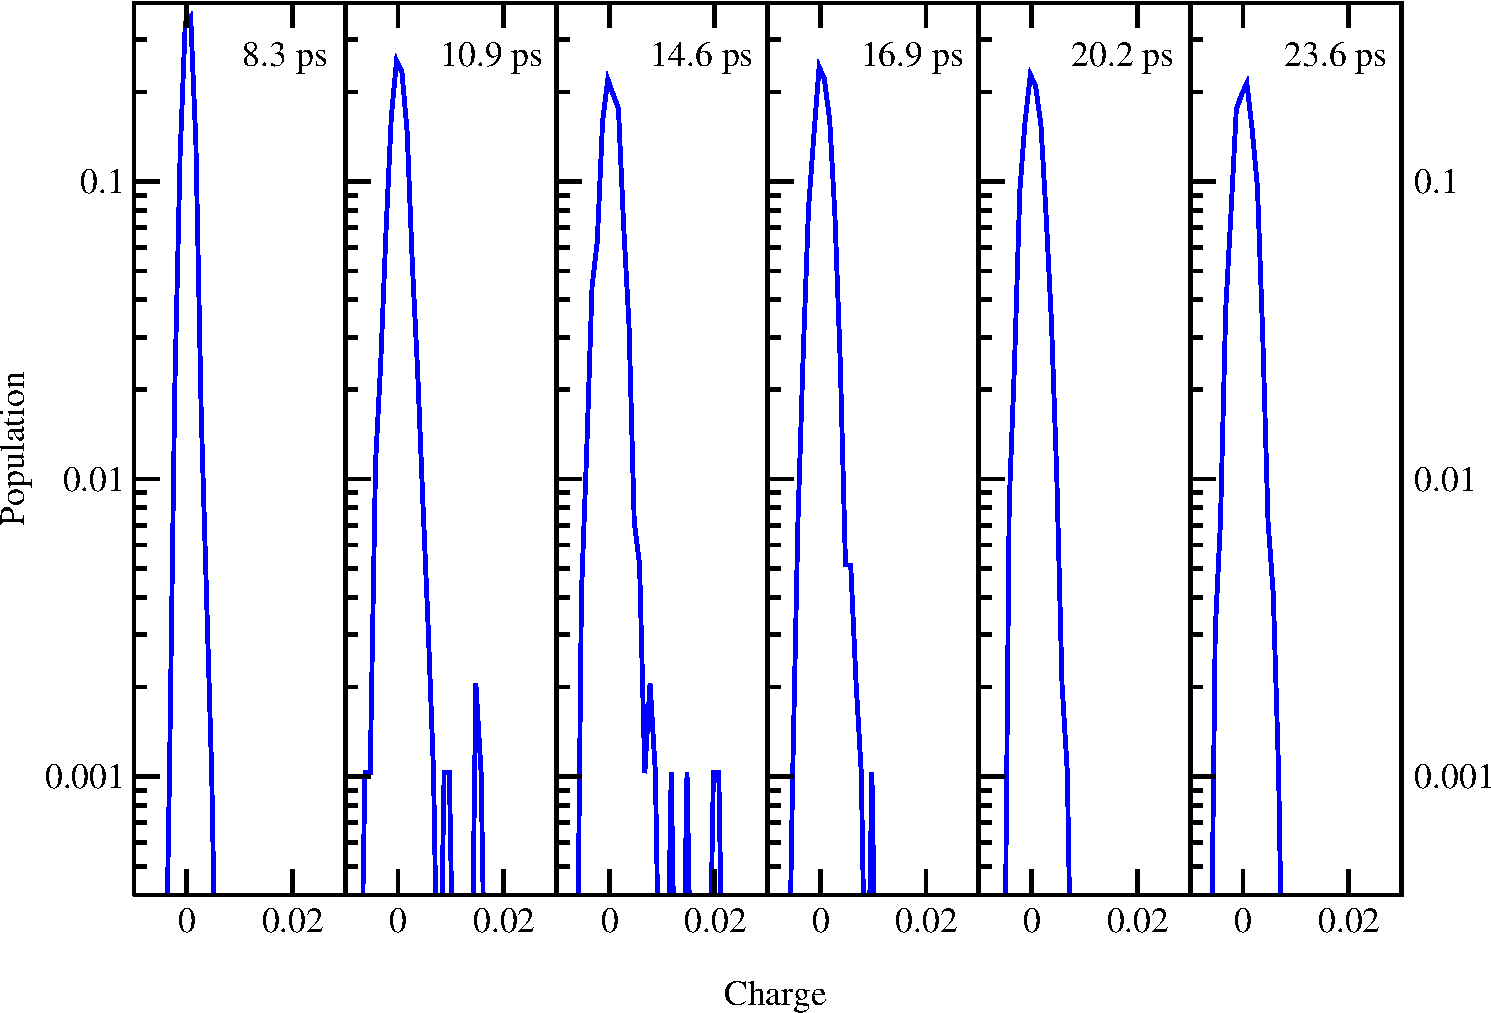
\includegraphics[width=0.9\linewidth]{../figures/chap5/frameChargeDistribution.pdf}
  \caption{Charge distributions in \ce{Pt} corresponding to the snapshots
depicted in Figure \ref{fig:chargeVol}. As the bulk of the metal is unaffected, a
logarithmic $y$-axis is utilized to highlight the atoms that deviate from 0
charge. As \ce{O-} approaches the surface, small peaks corresponding to surface
\ce{Pt} atoms with a slightly positive charge appear. As the charge is smeared
out over a handful of \ce{Pt} atoms, each one tends to approach 0.02 $e^-$.}
\label{fig:chargeHistogram}
\end{figure}

\section{Future directions}
While this method has succeeded in capturing the movement and accumulation of
charge in a metal surface in response to an incoming ion, accurate
parameterization of the numerous parameters is still on-going. Additionally,
the build-up of charge at the surface rather than at some depth $d$, appears to
be in violation of the method of images. Further work is thus needed to
properly incorporate the electrical potential being constant at the surface of
a conductor.  This work is on-going and when completed opens up a large realm
of possible directions of studies, specifically, oxide formation on platinum is
of immense interest. Additional interactions with metal surfaces will also be
explored with this technique and will include small molecules, {\em i.e.}
\ce{CO}, \ce{H2O}, \ce{NO}, etc., metal ions, and small biological analogs like
that amino acids and short peptide chains.



